
The general equation of circle is
\begin{align}
    \vec{x}^T\vec{x} - 2\vec{c}^T\vec{x} + f = 0
\end{align}
where $\vec{c}$ is the centre of the circle.
\begin{align}
    \vec{c} &= \myvec{3 \\ 2}\\
    \vec{O} &= \vec{c}\\
    \vec{M} &= \myvec{4 \\ 1}
\end{align}
The line passing through the centre bisects any chord perpendicularly. The direction vector of $\vec{O}\vec{M}$ is
\begin{align}
    \vec{OM} &= \vec{M} - \vec{O}\\
    &= \myvec{4 \\ 1} - \myvec{3 \\ 2}\\
    &= \myvec{1 \\ -1}
\end{align}
The normal vector $\vec{n}$ is
\begin{align}
    \vec{n} = \vec{OM}
\end{align}
The equation of line in terms of normal vector
\begin{align}
    \vec{n}^T(\vec{x} - \vec{M}) &= 0\\
    \myvec{1 & -1}\vec{x} &= \myvec{1 & -1}\vec{M}\\
    \myvec{1 & -1}\vec{x} &= \myvec{1 & -1}\myvec{4 \\ 1}\\
\implies     \myvec{1 & -1}\vec{x} &= 3
\end{align}
See Fig.     \ref{rams/4/2/18/fig:plot}
\begin{figure}[htp]
    \centering
    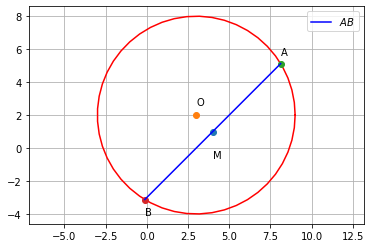
\includegraphics[width=\columnwidth]{solutions/4/2/18/Figures/Fig1.png}
    \caption{Plot of the given points and circle}
    \label{rams/4/2/18/fig:plot}
\end{figure}

